
\subsection{2.5. Устойчивость молекулы согласно методу молекулярных орбиталей. Сравнение предельных типов химической связи (ковалентная неполярная и ионная).} 

\par\bigskip

Согласно ММО, молекула устойчива, если кратность связи $\geq1$ (не всегда так).
	
\par\smallskip

\begin{figure}[H]
	\centering
	{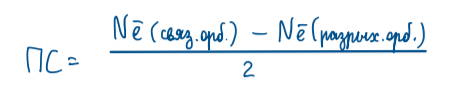
\includegraphics[scale=1]{7.png}}

\end{figure}

\par\smallskip
Несвязывающие орбитали не вносят вклад в порядок связи.
\par\smallskip


\begin{figure}[H]
	\centering
	{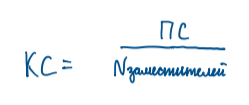
\includegraphics[scale=1]{8.png}}
\end{figure}

\begin{center}
$\Downarrow$

\par\smallskip
Для молекул типа ЭЭ’ ПС=КС

\end{center}


Так как разрыхляющие орбитали всегда больше разрыхляют,
чем связывающие связывают, то не должны существовать
системы, где число электронов на связывающих орбиталях
равно числу электронов на разрыхляющих орбиталях.

\par\smallskip

\begin{figure}[H]
	\centering
	{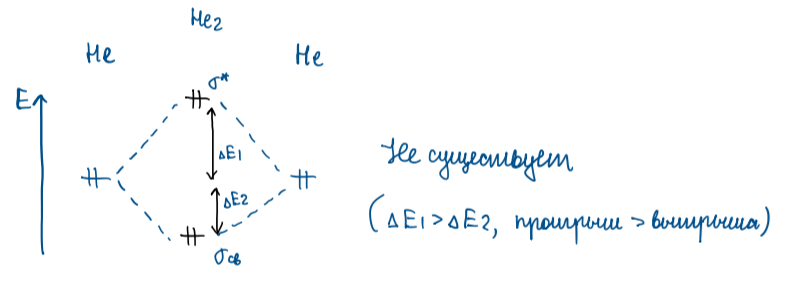
\includegraphics[scale=1]{9.png}}
\end{figure}

\par\smallskip

Тем не менее, могут быть устойчивы молекулы или ионы с КС $<1$ (1)
и неустойчивы молекулы или ионы с КС $\geq1$ (2).

\par\smallskip

(1) Это проявляется для систем с трёхцентровым перекрыванием.
Например, $3с4е$ - электроно-избыточное орбитально-дефицитное
$[HF2]^-$.

\par\smallskip

\begin{figure}[H]
	\centering
	{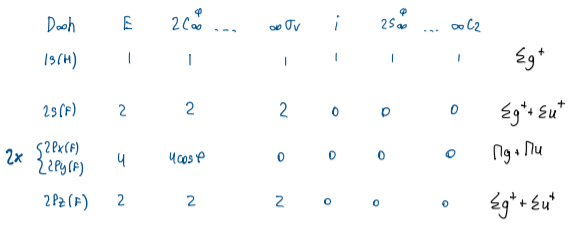
\includegraphics[scale=1]{10.png}}
\end{figure}

\par\smallskip

\par\smallskip

\begin{figure}[H]
	\centering
	{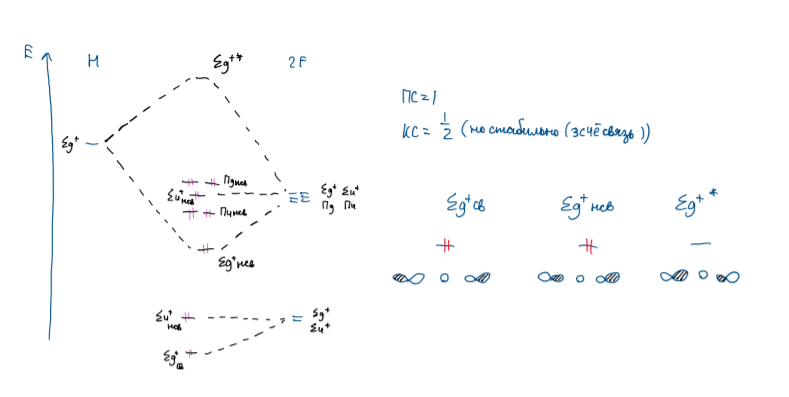
\includegraphics[scale=1]{11.png}}
\end{figure}

\par\smallskip

Полностью заполненная связывающая МО означает, что в молекуле
возникает связь, следовательно, она должна быть устойчива (КС
меньше 1, поскольку электронная пара находится не на двух-, а на
трехцентровой МО).

\par\smallskip

(2) Пример: $BH_3$ - очень сильная кислота Льюиса, в мономерном
состоянии неустойчива и при отсутствии доноров электронной
пары реагирует сама с собой с образованием димера $B_2H_6$.
	
\par\smallskip

\begin{figure}[H]
	\centering
	{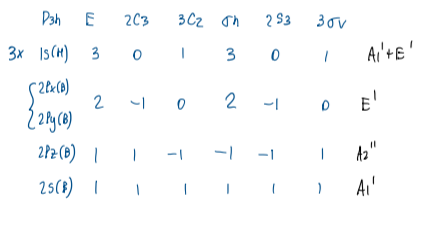
\includegraphics[scale=1]{12.png}}
\end{figure}


\begin{figure}[H]
	\centering
	{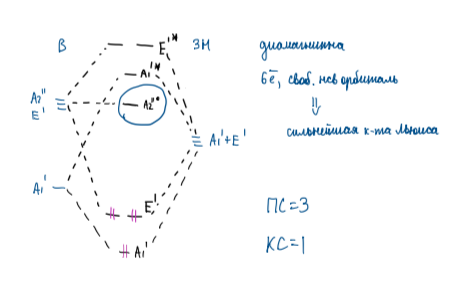
\includegraphics[scale=1]{13.png}}
\end{figure}

\par\smallskip
	
	\begin{center}
	\textbf{Сравнение ионной и ковалентной неполярной химических связей.}
	\end{center}
	
		\begin{figure}[H]
		\centering
		{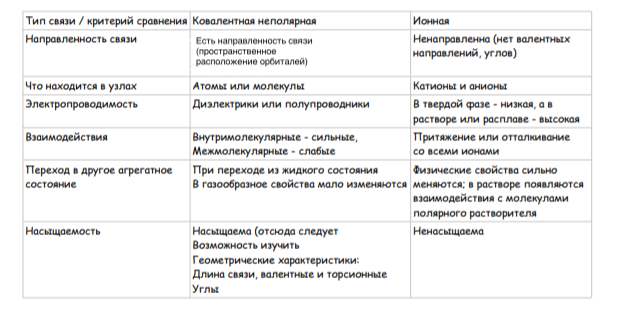
\includegraphics[scale=1.4]{14.png}}
	\end{figure}

\par\bigskip
\par\bigskip